\chapter{Spring security}

\fcolorbox{black}[HTML]{E9F0E9}{\parbox{\textwidth}{%
\noindent \textbf{Learning goals}\\
The junior-colleague
\begin{enumerate}[nolistsep]
\item todo
\end{enumerate}
}}


\fcolorbox{black}[HTML]{ADD8E6}{\parbox{\textwidth}{%
\noindent \textbf{Source for this chapter:}\\
\url{https://github.com/custersnele/PAJ_Demo_MockMvcWithSecurity.git}
}}


\section{What is spring security}

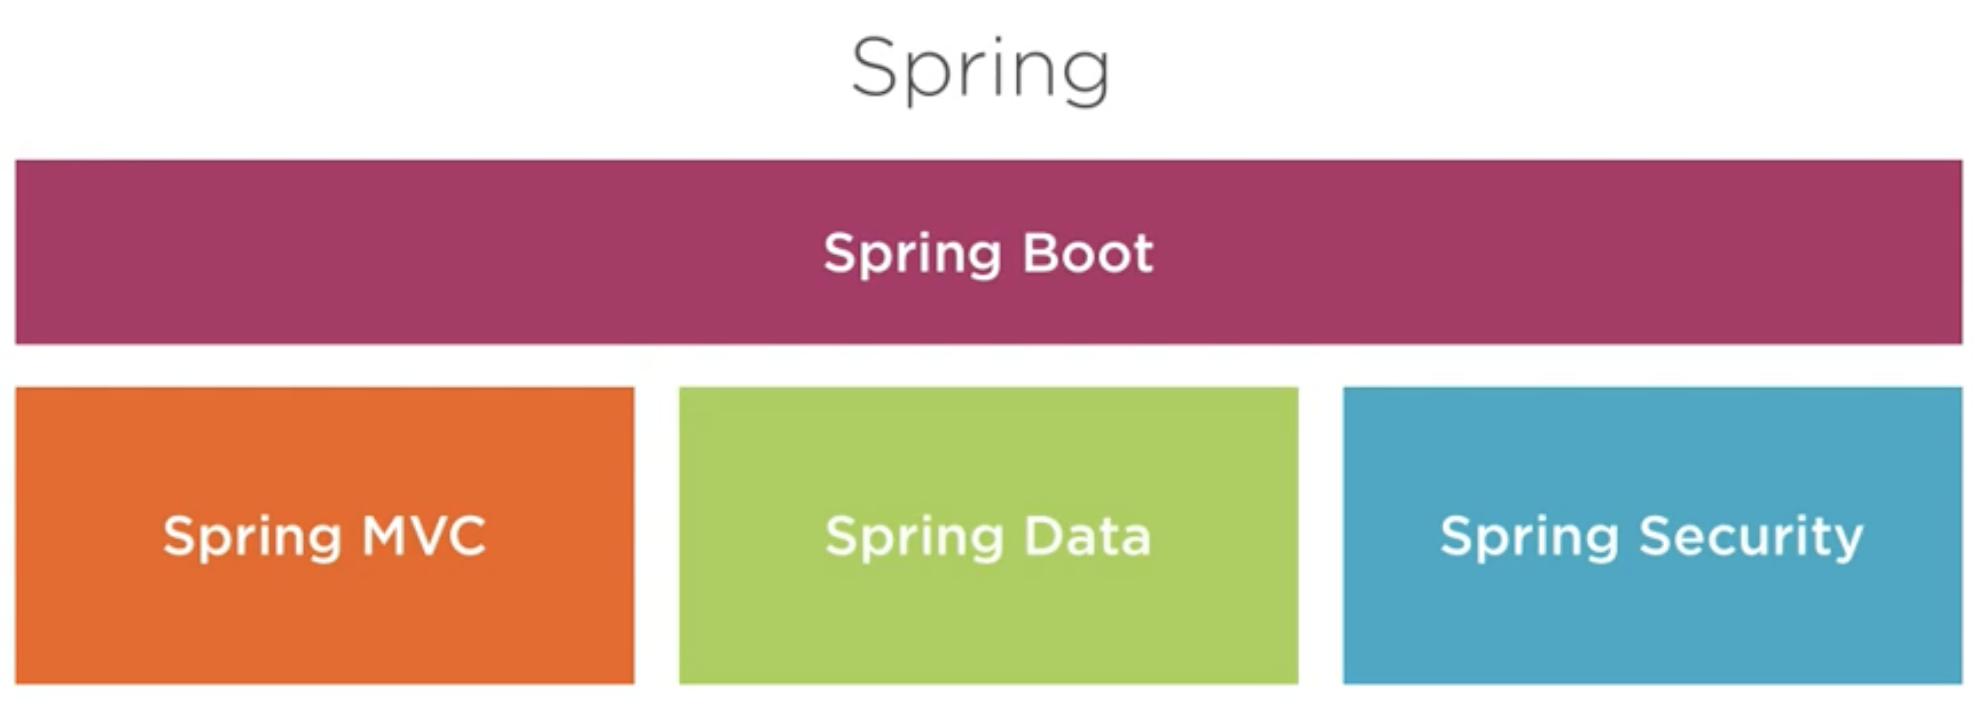
\includegraphics[width=\textwidth]{./images/chapter-tx/spring_boot.png}

Spring Security is a framework that provides authentication, authorization, and protection against common attacks.

\section{JWT tokens}

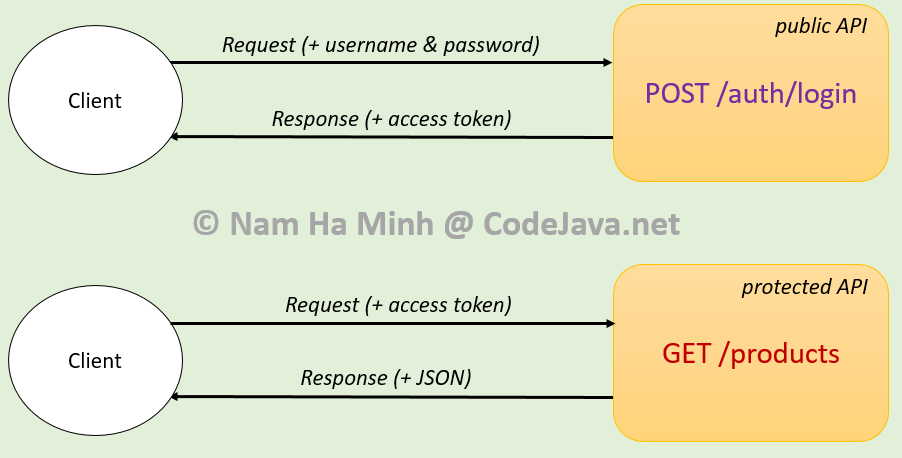
\includegraphics[width=\textwidth]{./images/chapter-tx/JWT_request_response.png}

\section{Implementation}

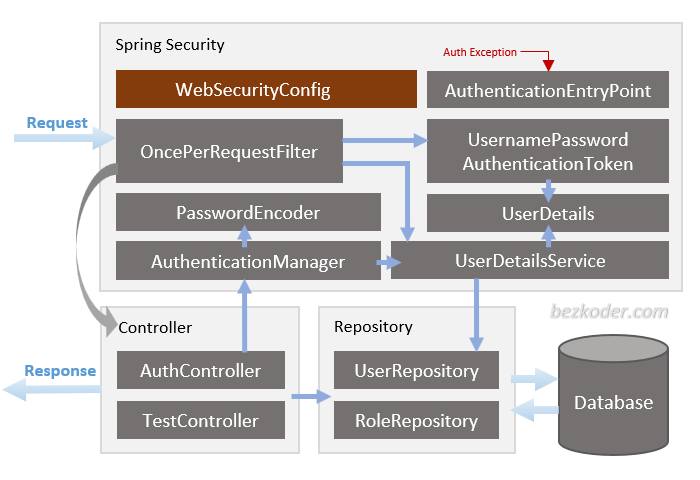
\includegraphics[width=\textwidth]{./images/chapter-tx/spring-boot-security-jwt.png}

To enable HTTP Security in Spring, we need to create a SecurityFilterChain bean.


\textbf{WebSecurityConfig} holds all security implementation details. It configures cors, csrf, session management, rules for protected resources. We can also extend and customize the default configuration that contains the elements below.
WebSecurityConfig used to extend WebSecurityConfigurerAdapter, but WebSecurityConfigurerAdapter is deprecated from Spring 2.7.0.


\textbf{UserDetailsService} interface has a method to load User by username and returns a UserDetails object that Spring Security can use for authentication and validation.

\textbf{UserDetails} contains necessary information (such as: username, password, authorities) to build an Authentication object.

\textbf{UsernamePasswordAuthenticationToken} gets {username, password} from login Request, AuthenticationManager will use it to authenticate a login account.

\textbf{AuthenticationManager} has a DaoAuthenticationProvider (with help of UserDetailsService and PasswordEncoder) to validate UsernamePasswordAuthenticationToken object. If successful, AuthenticationManager returns a fully populated Authentication object (including granted authorities).

\textbf{OncePerRequestFilter} makes a single execution for each request to our API. It provides a doFilterInternal() method that we will implement parsing and validating JWT, loading User details (using UserDetailsService), checking Authorization (using UsernamePasswordAuthenticationToken).

\textbf{AuthController} handles login (and signup) requests.

You can enable security debugging as follows:

\begin{lstlisting}
@EnableWebSecurity(debug = true)
public class SecurityConfiguration {
...
}
\end{lstlisting}

\section{Unit tests}

With the @SpringBootTest annotation, Spring Boot provides a convenient way to start up an application context to be used in a test.

\begin{lstlisting}
@BeforeEach
void setup() {
	mockMvc = MockMvcBuilders
			.webAppContextSetup(context)
			.apply(SecurityMockMvcConfigurers.springSecurity())
			.build();
}
\end{lstlisting}

When using @SpringBootTest annotation to test controllers with Spring Security, it's necessary to explicitly configure the filter chain when setting up MockMvc.

Using the static springSecurity method provided by  SecurityMockMvcConfigurer is the preferred way to do this.

The annotation @WithMockUser is used to mock a logged-in user.

\section{Enabling Actuators, Metrics, and Health Indicators}

Actuator brings production-ready features to our application.
Monitoring our app, gathering metrics, understanding traffic, or the state of our database become possible with this dependency.
The main benefit of this library is that we can get production-grade tools without having to actually implement these features ourselves.

\begin{lstlisting}
<dependency>
	<groupId>org.springframework.boot</groupId>
	<artifactId>spring-boot-starter-actuator</artifactId>
</dependency>
\end{lstlisting}

Actuator comes with most endpoints disabled, to enable all endpoints use the following property:

\begin{verbatim}
management.endpoints.web.exposure.include=*
\end{verbatim}

As you can see, there are endpoints provided by the Spring Boot Actuator that expose important information about the application. Carefully evaluate the need to bring in spring-boot-stater-actuator and take steps to minimize the risk of security attacks.






